\section{Measure}

\qs{General one qubit measure}
{
    Take the general form of an observable acting on a qubit $A = \vb{n}\vdot\vb*{\sigma}$, where $\vb*{\sigma}$ is a vector containing the Pauli matrices and $\vb{n}$ is real versor. Find out the possible outcomes of a measure done on a general state $\ket{\psi}$ and their probability of happening.

    At last, show how the measuring $A$ on the computational basis is not totally equivalent to measuring it in the $\ket{e_\pm}$ orthonormal base of eigenstates since $\ket{\psi}$ collapse in different states, but the following circuit
    \begin{center}
        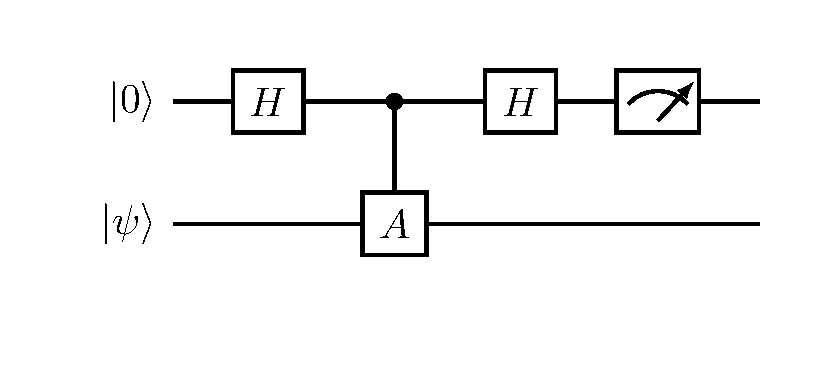
\includegraphics[width=0.7\textwidth]{Immagini/POVM.pdf}
    \end{center}
    can instead reproduce the exact measure by evaluating the axiliary qubit, forming the POVM of the $A$ PVM measure.
}
\pf{Solution}
{
    First we can easily find out the values of the eigenvalues by using the following trick. We can take the square of the matrix seeing how
    \begin{equation}
        \left( \vb{n}\vdot\vb*{\sigma} \right)^2 = n_x^2 X^2 + n_y^2 Y^2 + n_z^2Z^2 + n_xn_yXY + n_xn_yYX + \dots,
    \end{equation}
    by recalling that $XY = -YX$ for every couple of Pauli matrix and $X^2=Y^2=Z^2 = \mathbb{1}$ we can see how
    \begin{equation}
        \left( \vb{n}\vdot\vb*{\sigma} \right)^2 = \abs{\vb{n}}\mathbb{1} = \mathbb{1}.
    \end{equation}
    Therefore, we can say that the squares of the eigenvalues of $A$ needs to give $1$, but we can also say that the following is true
    \begin{equation}
        \trace{A} = n_x \trace{X} + n_y \trace{Y} + n_z\trace{Z} = 0.
    \end{equation}
    Meaning that we can now find out the eigenvalues of the matrix $\lambda_{\pm}$ simply by knowing that $\abs{\lambda_{\pm}}^2 = 1$ and that their sum needs to be zero $\lambda_+ + \lambda_- = 0$ having that the only possible solution is
    \begin{align}
        &\lambda_+ = +1, &\lambda_- = -1.
    \end{align}
    Meaning that the only possible outcomes of the measure is still $\pm 1$ also for this observable.

    Now, to measure the probability of one outcome to appear we need to write down the projector on the base of the observable. In particular, we can say that being $A$ selfadjoint a base $\ket{e_\pm}$ of eigenvector exist whose projectors $P_\pm = \ketbra{e_{\pm}}$ has the properties
    \begin{align}
        &\vb{n}\vdot\vb*{\sigma} = P_+ - P_-, &\mathbb{1} = P_+ + P_-.
    \end{align}
    Meaning that we can invert those and find out in the end the following forms
    \begin{equation}
        P_\pm = \frac{\mathbb{1} \pm A}{2}.
    \end{equation}
    From this we can easily write down the probabilities of measuring in a state like $\ket{\psi} = \alpha\ket{e_+} + \beta\ket{e_2}$ which are simply $p_+ = \abs{\alpha}^2$ and $p_- = \abs{\beta}^2$. Nevertheless, we are interested also in evaluating it in the computational base so that the state is written as  $\ket{\psi} = a\ket{0} + b\ket{1}$ having that the probability becomes
    \begin{equation}
        \tilde{p}_\pm = \ev{P_\pm}{\psi} = \frac{1}{2}\left[ (1\pm n_z) \pm 2n_x\Re{a^*b} \pm 2n_y\Im{a^*b} \right].
    \end{equation}
    Where one can see how the coefficients generate added terms to the probabilities in case of superpositioning, meaning that if one of the two $a$ or $b$ is zero the added terms vanishes. Also, those terms depends on the relative phase of the two coeffiecients meaning that \textbf{interference effects} can happen. Still, the values obtained are in reality equal to the one of $\alpha$ and $\beta$ squared seen previusly if one does all the computations, meaning that the probabilities evaluated in the two bases are the same. What changes is the collapsing since in the normal base $\ket{\psi}$ collapse in one of the two $\ket{e_\pm}$ while in the computational will become either $\ket{0}$ or $\ket{1}$.

    We can now see how the circuit we have seen that uses an auxiliary qubit to perform the computation is able to generate the exact measure we are searching for, also forming a POVM for that measure. To see that we can see how the state of the system evolves inside the circuit by starting from the application of the Hadamert gate and of the CA one having
    \begin{equation}
        \ket{0}\ket{\psi} = \frac{\ket{0}\ket{\psi} + \ket{1}A\ket{\psi}}{\sqrt{2}}.
    \end{equation}
    Then, by using a second Hadamart gate we can easily see how the state can be written simply as
    \begin{equation}
        \ket{0}\left( \frac{\mathbb{1} + A}{2} \right)\ket{\psi} + \ket{1}\left( \frac{\mathbb{1} - A}{2} \right)\ket{\psi} = \ket{0}P_+\ket{\psi} + \ket{1}P_-\ket{\psi}.
    \end{equation}
    Meaning that we have an entangled state where, by measuring the first qubit in the computational base allow us to know the state of $\ket{\psi}$ that has collapsed in one of the two eigenstate of $A$. Also, we can see how the probability of measuring the outcome $\pm 1$ in the computational base is given by
    \begin{equation}
        \braket{0}\ev{P_\pm^\dagger P_\pm}{\psi} = \tilde{p}_\pm.
    \end{equation}
    Basically the probabilities remains the same but now the states collapse in the right way so that the full measure is obtained, we only need one extra qubit.
}